% ****** Start of file apssamp.tex ******
%
%   This file is part of the APS files in the REVTeX 4.2 distribution.
%   Version 4.2a of REVTeX, December 2014
%
%   Copyright (c) 2014 The American Physical Society.
%
%   See the REVTeX 4 README file for restrictions and more information.
%
% TeX'ing this file requires that you have AMS-LaTeX 2.0 installed
% as well as the rest of the prerequisites for REVTeX 4.2
%
% See the REVTeX 4 README file
% It also requires running BibTeX. The commands are as follows:
%
%  1)  latex apssamp.tex
%  2)  bibtex apssamp
%  3)  latex apssamp.tex
%  4)  latex apssamp.tex
%
\documentclass[
 reprint,
linenumbers,
%superscriptaddress,
%groupedaddress,
%unsortedaddress, 
%superscriptaddress,
%groupedaddress,
%unsortedaddress,
%runinaddress,
%frontmatterverbose, 
%preprint,
%preprintnumbers,
%nofootinbib,
%nobibnotes,
%bibnotes,
aps,amsmath
%pra,
%prb,
%rmp,
%prstab,
%prstper,
%\floatfix,
]{revtex4-2}
\usepackage{graphicx}% Include figure files
\usepackage{dcolumn}% Align table columns on decimal point
\usepackage{bm}% bold math
\usepackage{adjustbox}
\usepackage{subfigure}
\usepackage[hidelinks]{hyperref}% add hypertext capabilities
\usepackage{braket}
%\usepackage[mathlines]{lineno}% Enable numbering of text and display math
%\linenumbers\relax % Commence numbering lines
%\usepackage[showframe,%Uncomment any one of the following lines to test 
%%scale=0.7, marginratio={1:1, 2:3}, ignoreall,% default settings
%%text={7in,10in},centering,
%%margin=1.5in,
%%total={6.5in,8.75in}, top=1.2in, left=0.9in, includefoot,
%%height=10in,a5paper,hmargin={3cm,0.8in},
%]{geometry}
\begin{document}
\preprint{APS/123-QED}

\title{Confirming the Total Angular Momentum of Rubidium:\\ 
An Optical Pumping Experiment}% Force line breaks with \\
%\thanks{A footnote to the article title}%

\author{Cameron Colucci}
 %\altaffiliation[Also at ]{Physics Department, XYZ University.}%Lines break automatically or can be forced with \\
%\author{Second Author}%
 %\email{Second.Author@institution.edu}
%\affiliation{%
 %Authors' institution and/or address\\
% This line break forced with \textbackslash\textbackslash
%}%

\collaboration{University of San Diego: Department of Physics}%\noaffiliation

%\author{Charlie Author}
 %\homepage{http://www.Second.institution.edu/~Charlie.Author}
%\affiliation{
% Second institution and/or address\\
% This line break forced% with \\
%}%
%\affiliation{
% Third institution, the second for Charlie Author
%}%
%\author{Delta Author}
%\affiliation{%
 %Authors' institution and/or address\\
 %This line break forced with \textbackslash\textbackslash
%}%

%\collaboration{CLEO Collaboration}%\noaffiliation

\date{\today}% It is always \today, today,
             %  but any date may be explicitly specified

\begin{abstract}
Abstract here

%\begin{description}
%\item[Usage]
%Secondary publications and information retrieval purposes.
%\item[Structure]
%You may use the \texttt{description} environment to structure your abstract;
%use the optional argument of the \verb+\item+ command to give the category of each item. 
%\end{description}
\end{abstract}

%\keywords{Suggested keywords}%Use showkeys class option if keyword
%display desired
\maketitle

%\tableofcontents

\section{\label{Intro}Introduction}%\protect\\ The line
%break was forced \lowercase{via} \textbackslash\textbackslash}

This paper uses optical pumping techniques to experimentally derive a numerical value of the total nuclear spin quantum number $I$, for Rubidium (Rb) isotopes 85 and 87. Optical pumping is a technique used in atomic physics to manipulate the population of atomic energy states through light absorption. When atoms are exposed to light at specific wavelengths, electrons in these atoms absorb photons and are excited from a lower energy state to a higher one. As these excited electrons return to lower energy states, they redistribute among the available magnetic sublevels differently from their initial distribution, which is influenced by the polarization of the light and the selection rules governing atomic transitions \cite{Optical_Pumping_Happer}. This technique is used in a variety of practical applications such as Magnetoencephalography \cite{MEG_example} and various laser technologies \cite{Laser_Example}. Among these practical applications, optical pumping is also used to discover, analyze, and confirm the characteristics of atoms and quantum mechanical systems, which is within the purpose of this paper. To support this paper's derivation of $I$, Sec. \ref{Theory} discusses the quantum theory needed to support this research, Sec. \ref{methods} outlines the experimental procedures followed to create the data, and Sec. \ref{results} presents the findings of the experiment.

\section{Theory} \label{Theory}

To fully understand this experiment, one must first be familiar with the selection rules that allow energy transitions in quantum mechanics. This experiment takes two different selection rules into account, electric dipole and magnetic dipole. Selection rules for energy transitions involve the quantum number $F$ which is defined as $F=I+J$, representing the total angular momentum. The electric dipole selection rules are derived from the necessity that the transition dipole moment must be non-zero for a transition to occur. For the dipole moment to be non-zero, it requires that the matrix element of the dipole operator between the two states have parity with the wavefunctions of the states involved \cite{McIntyre-QM,Foot_AtomicPhys}. These selection rules govern energy level transitions, such as what you would see on a typical energy level diagram. For electric dipole transitions, the permissible changes in these quantum states are dictated by $\Delta F = 0, \pm 1$, but in transitions where both the initial and final states have a $\Delta F = 0$, then the transition probability is zero and the transition is considered forbidden \cite{McIntyre-QM}. 

Although a transition may be considered forbidden by electric dipole selection rules, it may still be allowed by a higher-order interaction, specifically magnetic dipole interactions for this experiment. This introduces what is called the Zeeman effect, which is the coupling of an applied magnetic field to the nuclear magnetic moment which splits the $F$ states into magnetic sublevels \cite{McIntyre-QM_Zeeman}. These sublevels, the $m_F$ states, are allowed to transition by the magnetic dipole selection rules. The quantum number $m_F$ describes the projection of $F$ along the axis of an external magnetic field $\mathbf{B}$ has the states $\Delta m_F = 0, \pm F$ \cite{melissinos-mod-phys}. These different integer values are the orientations of $F$ about the magnetic field \cite{melissinos-mod-phys}. The magnetic dipole selection rules define the number of magnetic dipole transitions that can occur within a given energy state. For example, if $F=1$ then $m_F=0,\pm1$, and if $F=2$ then $m_F=0,\pm2$ and so on \cite{Foot_AtomicPhys}. It is important to take both of these selection rules into account, as both are necessary for understanding the characteristics of this experiment. 

The degree of splitting is influenced by the total nucleus angular momentum $I$, as it affects the total angular momentum by definition $F=I+J$ where $J$ is the total electron angular momentum. The combination of \(I\) and \(J\) leads to different splitting patterns in the presence of a magnetic field and can be observed through the process of optical pumping, which selectively populates specific magnetic sublevels \cite{McIntyre-QM_Zeeman, Optical_Pumping_Happer}. By diagonalizing the energy matrix for each Rb isotope, a Breit-Rabbi diagram can be created from the eigenvalues which display the electric and magnetic dipole energy corrections. One can see that as the magnetic field increases, the energy required to induce an electric dipole transition increases, but the magnetic dipole transition energy becomes constant. The full diagonalized matrix for $^{87}\mathrm{Rb}$ is shown below in a table due to the size of the matrix, and $^{85}\mathrm{Rb}$ (not shown) was diagonalized similarly.

\begin{table} [h]
\begin{tabular}{|c|c|}
\hline
$\mathbf{\ket{F, m_F}}$ & \textbf{Eigenvalue} \\ 
\hline \hline
$\mathbf{\ket{2,2}}$ & $3/4 \times A\hbar^2 + 1/2 \times g_J\mu_BB$ \\ \hline
$\mathbf{\ket{2,-2}}$ & $3/4 \times A\hbar^2 - 1/2 \times g_J\mu_BB$ \\ \hline
$\mathbf{\ket{2,1}}$ & $-1/4 \times A\hbar^2 - 1/2 \times \sqrt{4A^2\hbar^4 + g_J^2\mu_B^2B^2}$\\ \hline
$\mathbf{\ket{1,1}}$ & $-1/4 \times A\hbar^2 + 1/2 \times \sqrt{4A^2\hbar^4 + g_J^2\mu_B^2B^2}$\\ \hline
$\mathbf{\ket{2, 0}}$ & $-1/4 \times A\hbar^2 - \sqrt{4A^2\hbar^4 + 2A \times g_J\mu_BB\hbar^2 + g_J^2\mu_B^2B^2}$\\ \hline
$\mathbf{\ket{1,0}}$ & $-1/4 \times A\hbar^2 + \sqrt{4A^2\hbar^4 + 2A \times g_J\mu_BB\hbar^2 + g_J^2\mu_B^2B^2}$\\ \hline
$\mathbf{\ket{2,-1}}$ & $-1/4 \times A\hbar^2 - \sqrt{4A^2\hbar^4 - 2A \times g_F\mu_BB\hbar^2 + g_J^2\mu_B^2B^2}$ \\ \hline
$\mathbf{\ket{1,-1}}$ & $-1/4 \times A\hbar^2 + \sqrt{4A^2\hbar^4 - 2A \times g_F\mu_BB\hbar^2 + g_J^2\mu_B^2B^2}$\\ \hline
\end{tabular}
\caption{The diagonalized matrix of $^{87}\mathrm{Rb}$. These values are in order so that the top to bottom of the table reads left to right in the matrix. This depicts the $F$ states ($1$ and $2$) with the associated $m_F$ sublevels, and the energy eigenvalue for that state. All off-diagonal elements of this matrix are $0$.}
\label{Diag of Rb87}
\end{table}

By observing the splitting patterns, one can solve for $I$, and give a value for both $^{85}\mathrm{Rb}$ and $^{87}\mathrm{Rb}$. There are two ways that this experiment calculates the value of $I$. Experimentally, in the "weak field," the gyromagnetic ratio ($g_F$) can be used. The weak field is defined when the energy difference in magnetic sublevels is much less than the hyperfine splitting energy. This area is shown in FIGs. \ref{Rb 87 BRD} and \ref{Rb 85 BRD} as the small portion of lines before the quadratic curves. The relationship between $g_F$ and $I$ is expressed as

\begin{equation}
 g_F = g_J \frac{F(F+1) + J(J+1) - I(I+1)}{2F(F+1)},
 \label{EQ: g_F}
\end{equation}
where $g_J$ is the Lande g-factor and $J=1/2$ \cite{McIntyre-QM_Zeeman}. The Lande g-factor is defined as
\begin{equation}
    g_J=1+\frac{J(J+1)+S(S+1)-L(L+1)}{2J(J+1)},
\end{equation}
where $L$ is the orbital angular momentum and $S$ is the spin angular momentum \cite{McIntyre-QM_Zeeman}. For Rb, $g_J$ is calculated to be $2$, which we substitute into Eq. \ref{EQ: g_F}. This relationship can be used even if $F$ is unknown by plugging in the definition of $F$ discussed above. A value for $g_F$ can be experimentally measured by taking data from each isotope in the low field using optical pumping techniques and applying the relationship
\begin{equation}
    g_F=\frac{h\nu}{\mu_BB},
\end{equation}
where $\nu$ is the frequency, $h$ is Planck's constant, $B$ is the applied magnetic field, and $\mu_B$ is the Bohr magneton \cite{melissinos-mod-phys}. The data is plotted as frequency vs. magnetic field, showing a linear relationship in which the slope is $\nu/B$. This is used to solve $g_F$ for each isotope and then by applying that result to Eq. \ref{EQ: g_F}, the value of $I$ for both isotopes is calculated. It is important to note that the result for $I$ is quadratic, however only one result has relevance because $I$ is a positive integer or half-integer value by definition \cite{McIntyre-QM}.
\begin{figure} [h]
    \centering
    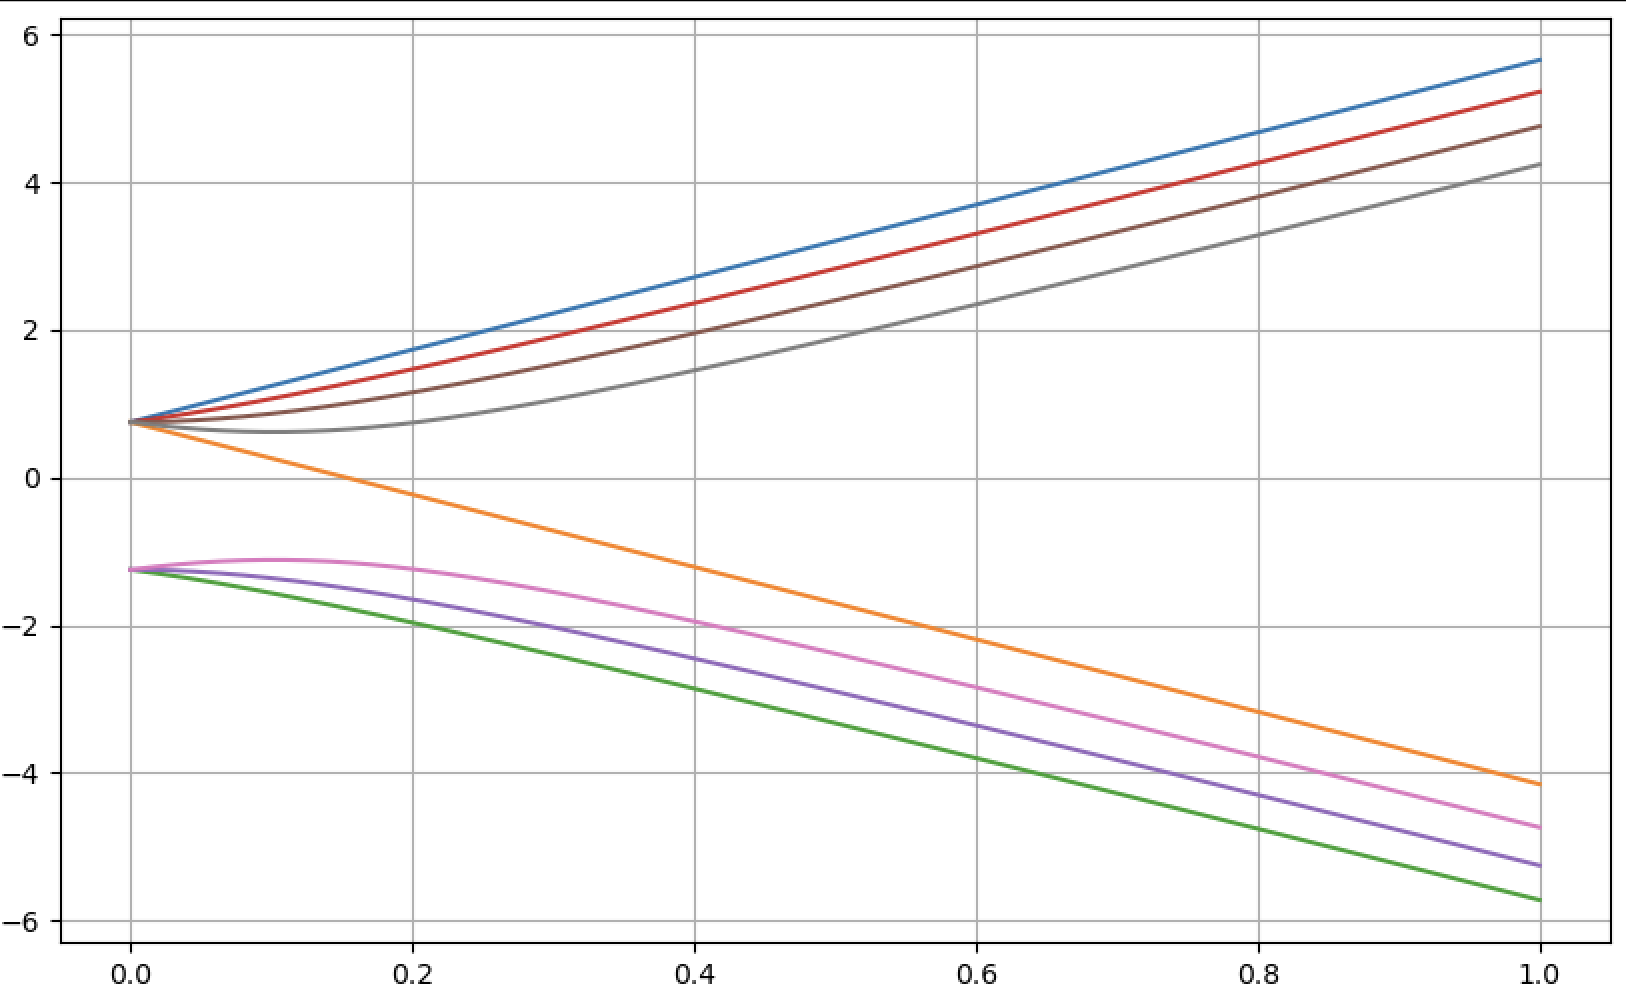
\includegraphics[width=1 \linewidth]{Images/Rb 87 BRD 3.png}
    \caption{Breit-Rabbi diagram for $^{87}\mathrm{Rb}$ created by plotting the diagonalized energy matrix, with unitless energy ($E/\Delta E$) on the y-axis and the external magnetic field $\mathbf{B}$ in Tesla on the x-axis. The top series of lines represents the $m_F$ states for the ground state $F=2$, and the lower series of lines are the $m_F$ states for the ground state $F=1$. The space between the two $F$ states represents the hyperfine splitting of the ground state.}
    \label{Rb 87 BRD}
\end{figure}

\begin{figure} [h]
    \centering
    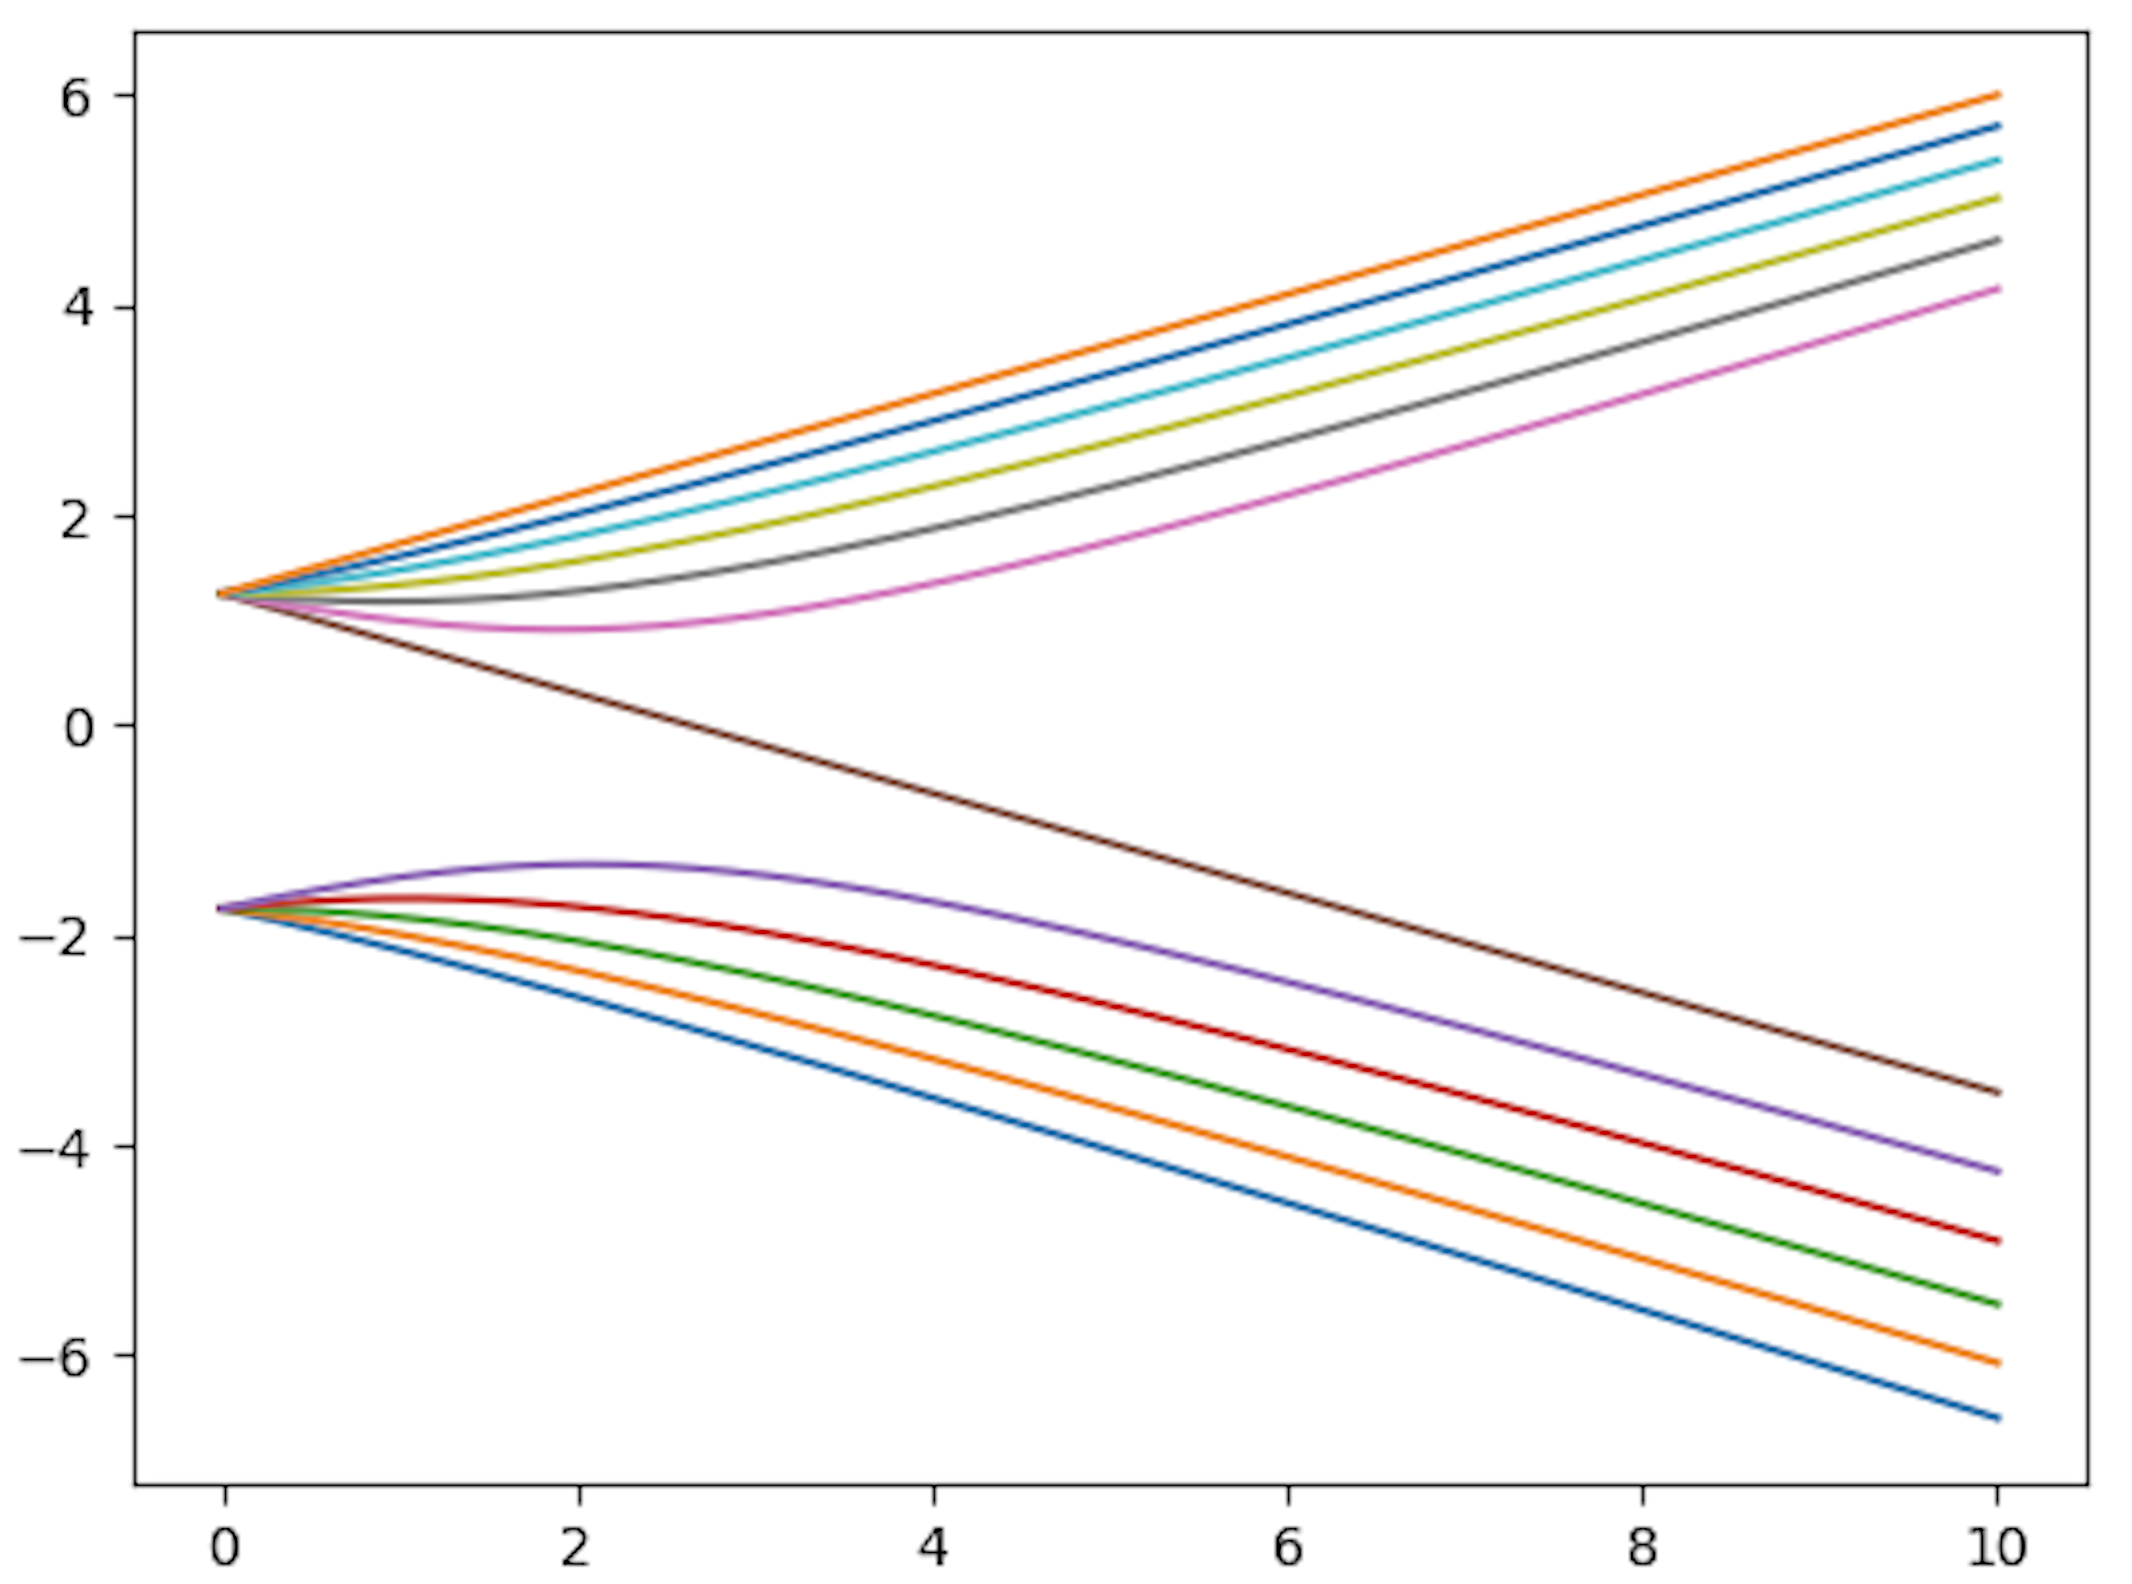
\includegraphics[width=1 \linewidth]{Images/Rb 85 BRD 2.png}
    \caption{Breit-Rabbi diagram for $^{85}\mathrm{Rb}$ created by plotting the diagonalized energy matrix, with unitless energy ($E/\Delta E$) on the y-axis and the external magnetic field $\mathbf{B}$ in Tesla on the x-axis. The top series of lines represents the $m_F$ states for the ground state $F=3$, and the lower series of lines are the $m_F$ states for the ground state $F=2$. The space between the two $F$ states represents the hyperfine splitting of the ground state.}
    \label{Rb 85 BRD}
\end{figure}

The other method for computing $I$ comes from the "high field", where the applied magnetic field is greater and the individual $m_F$ states can be visualized with optical pumping techniques. By counting the number of $m_F$ states shown from the data, $F$ can be determined by using the definitions above. By finding the value for $F$ and knowing that for Rb $J=1/2$, the relationship of $F=I+J$ can be used to directly solve for $I$ \cite{melissinos-mod-phys}.

\section{Experimental Methods} \label{methods}

\begin{figure*}
    \centering
    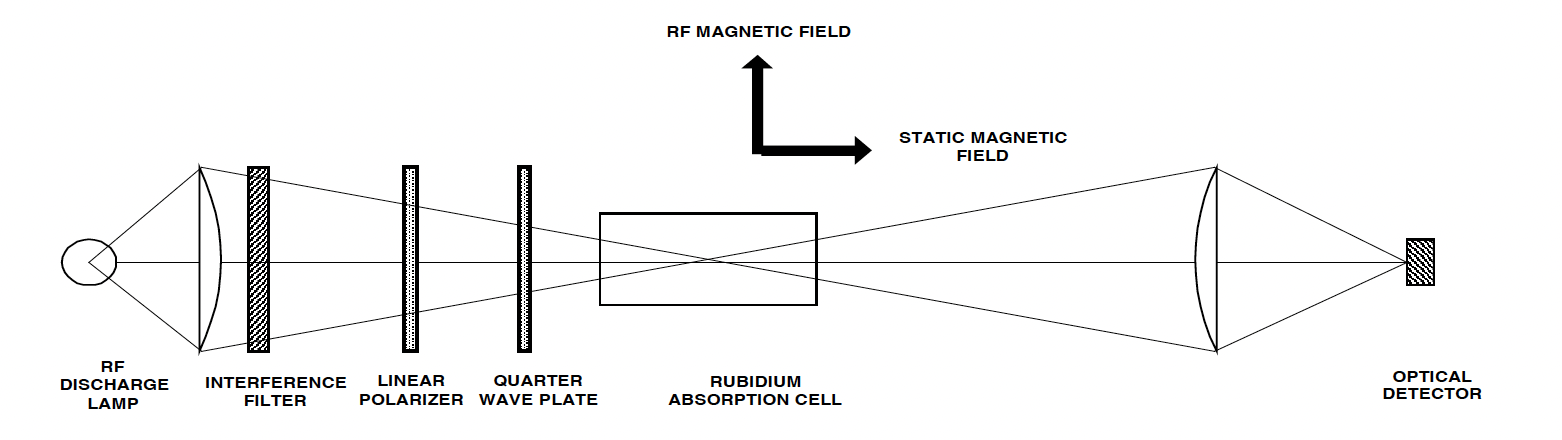
\includegraphics[width=1 \linewidth]{Images/Block Diagram.png}
    \caption{Block Diagram of Optical Pumping apparatus.}
    \label{Block Diagram}
\end{figure*}

This optical pumping experiment involves the Rb atom, with an $^5S_{1/2}$ ground state and a $^5P_{1/2}$ excited state. The atom is excited by optical radiation with exposure to right circularly polarized light that travels along an applied external RF magnetic field, $\mathbf{B}$. The right circularly polarized light ensures that atoms positively promote energy levels. For example, $F=1$ $m_F=-1$ in the ground state promotes an allowed excited state $m_F=0$. The atom then decays to the ground state at the same $m_F=0$ and absorbs RF light to promote again to an excited state $m_F=1$, and repeats this cycle. Atoms then reach a point where no further transitions are allowed by either of the selection rules described in Sec. \ref{Theory}, and a state of "transparency" occurs. Transparency in this case means that the atoms can no longer absorb the RF light, so all of the light passes through the Rb gas cell into the photodetector \cite{Optical_Pumping_Happer}.

The RF light is created by an Rb discharge lamp consisting of and an RF oscillator, a glass bulb of Rb vapor, and an oven. The Rb vapor in the bulb is heated so that the vapor pressure is increased. The oven temperature setting for this experiment is $50^\circ$ C for all data sets. A plano-convex lens is then placed in the apparatus just after the RF lamp to minimize spherical aberrations. After the first plano-convex lens near the RF lamp, an interference filter is placed that is tuned to $795$ nm allowing only the of that wavelength into the Rb cell, which is the D-line of interest in this experiment. Next, a linear polarizer and quarter-wave plate are placed which right circularly polarized the light before it is introduced into the Rb cell. After the light passes through the Rb cell, a second plano-convex lens is placed to collect the light and focus it onto the detector. The detector for this apparatus is a silicon photodiode, connected to the voltage preamplifier which collects the RF light that passes through the Rb cell. The external magnetic field supplied in this experiment is created by Helmholtz coils which induce a horizontal field, a vertical field, and a horizontal sweep field. The vertical magnetic field cancels the magnetic field of the earth, while the horizontal magnetic fields induce the Zeeman effect for data collection. It is also important to note that all of the induced magnetic fields are unipolar \cite{Optical_Pumping_Happer}.

Data collection consists of two separate sets, low field resonance and high field resonance. As discussed in Sec. \ref{Theory}, low field resonance occurs when the Rb cell is subjected to a weak external magnetic field. It is important to note that the magnetic field measurements in this experiment are in units of gauss. The vertical magnetic field remains fixed and the horizontal magnetic field is adjusted until small dips appear on the oscilloscope. By adjusting the settings on the oscilloscope, the spacing of the dips shift closer together or farther apart, depending on the data that is to be viewed. The low field resonance should appear as a series of three dips, one very large and two smaller dips. These dips in the graph represent a decrease in light intensity, meaning that light is being absorb at that particular magnetic field strength. The large dip represents the zero field transition, which represents the energy levels near a zero magnetic field. This dip is much larger than the others because at the zero field the energy levels become degenerate and much more light is absorbed by the Rb cell \cite{Foot_AtomicPhys}. The two smaller dips are the Zeeman resonances of the two isotopes, $^85\mathrm{Rb}$ and $^87\mathrm{Rb}$. The data collected from the low field resonance ranged from a $40$ kHz to $140$ kHz frequency setting with each data set increasing by $10$ kHz and captured using an active MATLAB script.

The high field resonance data was then observed by focusing on the zero field transition, and then adjusting the horizontal sweep field to "zoom in" on the individual isotope dips. Once a good image was established,

\section{Analysis and Results} \label{results}


\section{Conclusion} \label{conclusion}


% \begin{acknowledgments}
% We wish to acknowledge the support of the author community in using
% REV\TeX{}, offering suggestions and encouragement, testing new versions,
% \dots.
% \end{acknowledgments}

%To start the appendixes, use the \verb+\appendix+ command.
%This signals that all following section commands refer to appendixes
%instead of regular sections. Therefore, the \verb+\appendix+ command
%should be used only once---to setup the section commands to act as
%appendixes. Thereafter normal section commands are used. The heading
%for a section can be left empty. For example,
%\begin{verbatim}
%\appendix
%\section{Raw Data}
%\end{verbatim}
%will produce an appendix heading that says ``APPENDIX A'' and
%\begin{verbatim}
\appendix
%\section{Background}
%\end{verbatim}
%will produce an appendix heading that says ``APPENDIX A: BACKGROUND''
%(note that the colon is set automatically).
% \newpage

% \subsection{Diagonalized Matrices of Rb Isotopes}

% \begin{equation}

% \rotatebox{90}{$\begin{bmatrix}
% \frac{3}{4}A\hbar^2+\frac{1}{2}g_J\mu_BB & 0 & 0 & 0 & 0 & 0 & 0 & 0 \\
% 0 & \frac{3}{4}A\hbar^2-\frac{1}{2}g_J\mu_BB & 0 & 0 & 0 & 0 & 0 & 0 \\
% 0 & 0 & -\frac{\sqrt{3}}{4}g_J\mu_BB & 0 & 0 & 0 & 0 & 0 \\
% 0 & 0 & 0 & \frac{3}{4}A\hbar^2+\frac{1}{4}g_J\mu_BB & 0 & 0 & 0 & 0 \\
% 0 & 0 & 0 & 0 & -\frac{1}{4}A\hbar^2-\frac{1}{2}\sqrt{4A^2\hbar^4+g_J^2\mu_B^2B^2} & 0 & 0 & 0 \\
% 0 & 0 & 0 & 0 & 0 & -\frac{1}{4}A\hbar^2+\frac{1}{2}\sqrt{4A^2\hbar^4+g_J^2\mu_B^2B^2} & 0 & 0 \\
% 0 & 0 & 0 & 0 & 0 & 0 & -\frac{\sqrt{3}}{4}g_J\mu_BB & 0 \\
% 0 & 0 & 0 & 0 & 0 & 0 & 0 & -\frac{5}{4}A\hbar^2+\frac{1}{4}g_J\mu_BB \end{bmatrix}$}
% \end{equation}

%You can use a subsection or subsubsection in an appendix. Note the
%numbering: we are now in Appendix~\ref{app:subsec}.


% The \nocite command causes all entries in a bibliography to be printed out
% whether or not they are actually referenced in the text. This is appropriate
% for the sample file to show the different styles of references, but authors
% most likely will not want to use it.
%\nocite{*}
\bibliography{Ref}% Produces the bibliography via BibTeX.

\end{document}
%
% ****** End of file apssamp.tex ******
